% Advanced template for the submission to Econometrica journal.
% This template is suggested when *hyperref* package is used.
%
%Author: In this template, the places where you need to add information
%        (or delete line) are indicated by {???}.  Mostly the information
%        required is obvious, but some explanations are given in lines starting
%
%Author:
%All other lines should be ignored.  After editing, there should be
%no instances of ??? after this line.

% use option [draft] for initial submission;
%            [final] for the prepublication;


\documentclass[pdftex]{article}
\usepackage{xspace,amsmath,graphicx,graphics,hypernat,xcolor}
\usepackage{amsthm}
%\startlocaldefs
\newcommand{\etal}{{\it et~al.}\ }
\newcommand{\ie}{{\it i.e.}\ }
\newcommand{\eg}{{\it e.g.}\ }
\newcommand{\etc}{{\it etc.}\ }
\newcommand{\cf}{{\it cf.}\ }
\newcommand{\Ito}{It\^{o}\xspace}
\newcommand{\pa}{{\it p.a.}\xspace}
\newcommand{\psa}{\ensuremath{{\text{year}}^{-1/2}}\xspace}

%List of symbols shortcuts
% For command names that already exist, prepend a "G" (for "Glossary")

\newcommand{\ave}[1]{\left\langle#1 \right\rangle}
\newcommand{\tave}[1]{\overline{#1}}
\newcommand{\latinword}[1]{\textsf{\itshape #1}}
%\newcommand{\person}[1]{{\sc{#1}}}
\newcommand{\person}[1]{#1} % switched off because not used consistently
%\newcommand{\quote}[1]{{\it ``#1''}}
\newcommand{\bi}{\begin{itemize}}
\newcommand{\ei}{\end{itemize}}

\newcommand{\elabel}[1]{\label{eq:#1}}
\newcommand{\eref}[1]{(Eq.~\ref{eq:#1})}
\newcommand{\Eref}[1]{Equation~(\ref{eq:#1})}

\newcommand{\ceref}[2]{(\ref{eq:#1}#2)}

\newcommand{\tlabel}[1]{\label{tab:#1}}
\newcommand{\tref}[1]{(Table~\ref{tab:#1})}

\newcommand{\flabel}[1]{\label{fig:#1}}
\newcommand{\fref}[1]{Fig.~\ref{fig:#1}}
\newcommand{\Fref}[1]{Figure ~\ref{fig:#1}}

\newcommand{\seclabel}[1]{\label{section:#1}}
\newcommand{\secref}[1]{Sec.~\ref{section:#1}}
\newcommand{\Secref}[1]{Section~\ref{section:#1}}

\newcommand{\clabel}[1]{\label{chapter:#1}}
\newcommand{\cref}[1]{Chap.~\ref{chapter:#1}}
\newcommand{\Cref}[1]{Chapter~\ref{chapter:#1}}



\newcommand{\OP}[1]{{\bf @@@OP: #1 @@@}}
\renewcommand{\AA}[1]{{\bf ===AA: #1 ===}}

\newcommand{\eq}{\hspace{-.15cm}=\hspace{-.15cm}}
\newcommand{\dist}{\,{\buildrel d \over =}\,}
\newcommand{\be}{\begin{equation}}
\newcommand{\ee}{\end{equation}}
\newcommand{\bea}{\begin{eqnarray}}
\newcommand{\eea}{\end{eqnarray}}
\newcommand{\bc}{\begin{center}}
\newcommand{\ec}{\end{center}}
\newcommand{\prob}[1]{\mathcal{P}\left(#1\right)}
\newcommand{\DW}{{\Delta W}}
\newcommand{\Dx}{{\Delta x}}
\newcommand{\DX}{{\Delta X}}
\newcommand{\Du}{\Delta u}
\newcommand{\tm}{{f_{\text{\normalfont{m}}}}}
\newcommand{\tml}{{f_{\text{\normalfont{m}}}^{\text{\normalfont{U}}}}}
\newcommand{\tmb}{{f_{\text{\normalfont{m}}}^{\text{\normalfont{B}}}}}
\newcommand{\dW}{{\delta W}}
\newcommand{\gbar}{\bar{g}}
\newcommand{\nn}{\nonumber}

% load additional packages:
%\usepackage{amsthm,amsmath,natbib}
%\RequirePackage[colorlinks,citecolor=blue,urlcolor=blue]{hyperref}

% use this package if hyperref and natbib is used:
%\RequirePackage{hypernat}

% put your definitions there:
%\endlocaldefs

\begin{document}

%\begin{frontmatter}

% "Title of the paper"
\title{Comment on D. Bernoulli (1738)}
\author{Ole Peters\\
\\
{\small London Mathematical Laboratory, 8 Margravine Gardens, London W6 8RH, UK}\\
{\small Santa Fe Institute, 1399 Hyde Park Road, Santa Fe, 87501 NM, USA}\\
{\small o.peters@lml.org.uk}}
\maketitle

%\runauthor{O. Peters}

\begin{abstract}
Daniel Bernoulli's study of 1738 is considered the birthplace of expected utility theory. Due to its central importance in economics, a translation from Latin to English was published in 1954 by L. Sommer \cite{Bernoulli1738}. Bernoulli's study stands at the very beginning of formal economic theory, when key concepts were being invented and had not yet settled into their modern form. Here I point out an inconsistency between the theory put forward by Bernoulli and modern expected-utility theory. 
\end{abstract}
%\begin{keyword}
%\kwd{}
%\kwd{}
%\end{keyword}

%\end{frontmatter}
\section{Preview}
Readers familiar with the context may start with \secref{Bernoullis}, skipping \secref{Historical} to \secref{Early}, which are included to ensure completeness and clarity of nomenclature. \Secref{Historical} is a very brief positioning of Bernoulli's study in its historical context. \Secref{Mathematical} makes explicit what we mean by a random variable and an expectation value. In \secref{Early}, both the earliest decision theory (expected-wealth maximization) and the currently most dominant form of decision theory (expected utility theory) are defined for reference. \Secref{Bernoullis} is the core result -- an exposition of the inconsistency between today's expected-utility theory and the decision theory originally put forward by Bernoulli. In \secref{Discussion} possible reasons for and consequences of Bernoulli's inconsistency are discussed.
 
\section{Historical positioning}
\seclabel{Historical}
Until the late 17th century it was generally believed that humans, when faced with the choice between two gambles of equal duration\footnote{I will disregard matters of time and discounting here, as they were not considered in Bernoulli's early work, which is the focus of the present study. My perspective on these problems is elaborated in \cite{PetersGell-Mann2016}.} will choose the one that possesses the larger expected wealth change. This earliest decision theory is well summarized by C. Huygens's statement ``if any one should put 3 shillings in one hand without telling me which, and 7 in the other, and give me choice of either of them; I say, it is the same thing as if he should give me 5 shillings...'' \cite{Huygens1657}. We will refer to this as ``Huygens's decision theory'' (HDT). 

In the early 18th century doubts were raised about the realism of this mathematical model of human behavior. Humans do not generally choose the gamble with the largest expected wealth change. In particular, Nicholas Bernoulli introduced the so-called St.~Petersburg gamble, in a letter to Montmort \cite[p.~402]{Montmort1713}, whose expectation value is divergent, \ie does not exist. How should such a gamble be evaluated?

Expected utility theory emerged out of ideas put forward by Cramer (cited in Bernoulli's 1738 paper) and Daniel Bernoulli, in response to these doubts about HDT. It is a means of accounting for the fact that people do not optimize expected wealth changes when evaluating gambles. We will distinguish between Bernoulli's decision theory (BDT) and what we mean today by ``expected utility theory'' (EUT). Although \cite{Bernoulli1738} is considered the beginning of EUT, it does not actually contain EUT as it is understood today.

An alternative modern accounting for the failure of HDT, using concepts that had not been developed by Bernoulli's time, is presented in \cite{PetersGell-Mann2016}. This modern perspective, based on ergodic theory, allows a deep understanding of Bernoulli's work and brought to light the inconsistency between BDT and EUT that we are about to discuss.

\section{Random variable and expectation value}
\seclabel{Mathematical}
For our discussion, we will need two concepts. Different authors favor slightly different nomenclatures, so for the avoidance of doubt I will define explicitly the terms used in this comment. The required concepts are: first a discrete random variable, and second the expectation value. 

\underline{Discrete random variable}\\
A discrete random variable is an object $Y$, defined by 
\bi
\item
a set of possible values, $\{y_i\}$, labelled with a number $i$, often called the $i^{\text{th}}$ event. 
\item
a set of probabilities, $\{P_Y(y_i)=p_i\}$, associated with these values.
\ei
The probabilities are non-negative, $p_i\geq0$ and add up to one,
\be
\sum_i p_i =1.
\ee
A function $z(y)$ defines another random variable, $Z$, whose set of possible values are the values of the function $z_i=z(y_i)$ at the possible values $y_i$ of the original random variable, $Y$. Its probabilities are also those of the corresponding events, $P_Z(z_i)=p_i$.

\underline{Expectation value}\\
The expectation value of a random variable, $\ave{y}_{P_Y}$, is the sum over the products of all possible values and their probabilities, 
\be
\ave{y}_{P_Y}=\sum_i y_i P_Y(y_i).
\ee
The operator $\ave{\cdot}$ is a simple (linear) sum. As a consequence, if $z(y)$ is a linear function of $y$, then the expectation values $\ave{z}_{P_Z}$ and
$\ave{y}_{P_Y}$ are trivially related, namely $\ave{z}_{P_Z}=z\left(\ave{y}_{P_Y}\right)$. 
This is easily proved
\begin{proof}
\bea
\text{Assume \hspace{.2cm}} z(y)&=&a y +b. \elabel{condition}\\
\text{Then \hspace{.1cm}}\ave{z}_{P_Z}&=& \sum_{i}p_i (a y_i + b)\\
&=&a \left(\sum_{i}p_i  y_i\right) + b\\
&=& z\left(\ave{y}_{P_Y}\right)
\eea
\end{proof}
If Huygens's statement had been restricted to linear $z(y)$, it would have been correct: in that case, it really is ``the same thing'' to consider the full distribution of $y$ as it is to work with its expecation value. 
Crucially, however without linearity, \eref{condition}, this trivial relationship does not hold. In other words, $\ave{z}_{P_Z}=z\left(\ave{y}_{P_Y}\right)$ implies linearity of $z(y)$. This is also easily proved
\begin{proof}
Assume
\bea
\ave{z}_{P_Z}&=&z\left(\ave{y}_{P_Y}\right)\\
\sum_{i}p_i z(y_i) &=& z\left(\sum_{i}p_i(y_i) \right)
\eea
Since the equation has to hold for general $y_i$, it has to hold term by term, and we have
\be
p_i z(y_i) = z (p_i y_i)
\ee
Differentiating with respect to $y_i$ yields
\bea
p_i z'(y_i) &=& p_i z' (p_i y_i)\\
z'(y_i) &=& z' (p_i y_i)
\eea
Again, since the equation has to hold for any $y_i$ it implies a constant first derivative of $z(y)$, which means $z(y)$ is linear.
\end{proof}

Therefore, Huygens's statement is not true: in general the random variable $Y$ is not ``the same thing'' as its expectation value $\ave{Y}$. However, because many functions $z(y)$ are linearizable for small changes in their arguments, researchers in the early days of probability theory were not fully aware of this complication.

\section{Early and late decision theories}
\seclabel{Early}
We model wealth as a number of dollars, $x$, and a gamble as a random variable, $\DX$, whose possible values, $\{\Dx_i\}$, represent the possible dollar-changes in wealth resulting from participating in the gamble. For example, consider a coin toss: we have to pay a \$1 fee to participate, if the coin lands tails we receive nothing, if it lands heads we receive \$3. This would be modelled as a random variable with two discrete possible values, $\Dx_1=-\$1$ (net change in wealth if the coin shows tails, we receive nothing but have paid the fee) and $\Dx_2=+\$2$ (net change in wealth if the coin shows heads). The probabilities would be $P_\DX(\Dx_1)=P_\DX(\Dx_2)=0.5$.

In general, we have a gamble modeled by some random variable $\DX$.

\subsection{Huygens's decision theory}
Imagine now deciding whether to participate in a gamble. This amounts to a comparison between no change in wealth (non-participation, which is a trivial gamble, sometimes called the null-gamble) and some evaluation of the random variable $\DX$. The evaluation of $\DX$ in HDT was $\ave{\Dx}$: the gamble is evaluated by comparing $\ave{\Dx}$ to 0. If $\ave{\Dx}>0$ (like in the example), this decision theory predicts that people will accept the gamble, if $\ave{\Dx}<0$ the prediction is non-participation.

Following discussions in the early 18th century \cite[p.~402]{Montmort1713}, it became clear that this decision theory is not a realistic model of human behavior, and expected-utility theory was developed as a better fit to the observations. We will come to Bernoulli's theory in the next section. First, I present today's standard EUT, almost exclusively in use at least since Laplace's early book on then-nascent probability theory \cite{Laplace1814}. 

\subsection{Expected utility theory}
Instead of maximizing $\ave{\Dx}$ in the choice of gambles, it appears that humans in their decisions maximize the expected change of a different random variable. Wealth is mapped into utility of wealth $u(x)$, and human decisions are now modeled as maximizing the expected change in utility, 
\be
\ave{\Du(x)}=\ave{u(x+\Dx)}-u(x).
\elabel{EUT}
\ee
This is a different mathematical model of human behavior. Crucially, EUT is sensitive to a reference level: wealth before the gamble, which we call $x_0$, unless the utility function is linear\footnote{To see this, require that $\Du$ be a function of $\Dx$ only, $u(x+\Dx)-u(x)=f(\Dx)$. Now imagine fixing $\Dx$ and varying $x$: the equation then implies that changes in the function in response to a change in the argument are constant, $\frac{du}{dx}=\text{const.}$, whose solution is a linear function $u(x)=ax+b$.} (which is not an interesting case because it predicts the same human behavior as maximizing $\ave{\Dx}$).

EUT thus introduces into decision theory the intuitively plausible notion that our ability and willingness to risk losing resources depends on the resources we have. A millionnaire may not notice the loss of \$1,000, whereas for someone else this may mean missing a year of school.

\underline{Summary:} EUT, as presented in countless textbooks, at least since \cite{Laplace1814}, models human decision-making by mapping wealth to utility $u(x)$. It then posits that decisions are made by selecting the gamble with the maximum expected change in utility.

\section{Bernoulli's decision theory is different}
\seclabel{Bernoullis}
Laplace, in 1814, and many authors after him, present EUT as I have done above. Laplace ascribes this fully to Bernoulli and does not mention that Bernoulli actually wrote something else. 

Bernoulli considers a gamble where a fee is paid, and prizes are received with different probabilities. He uses a cumbersome geometric notation which we replace with a more modern one, see \tref{key} and \fref{key}.

\begin{center}
\begin{table}
  \begin{tabular}{ l | c | c }
    \hline
    Object & Bernoulli's notation & Our notation \\ \hline
    Wealth before the gamble & AB & $x_0$ \\
    Maximum ticket fee in Bernoulli's theory & pB & $\tmb$ \\
    Maximum ticket fee in EUT & no symbol & $\tml$ \\
    Minimum prize received & BC & $\pi_1$\\
    2nd-smallest prize & BD & $\pi_2$\\
    3rd-smallest prize & BE & $\pi_3$\\
    4th-smallest prize & BF & $\pi_4$\\
    Utility change due to loss of maximum fee & po=An &$\Du^{-}$\\
    Utility change due to gain of expected prize & PO=AN&$\Du^+$\\
Probability of $\pi_1$ &$\frac{m}{m+n+p+q+\cdots}$&$p_1$\\
Probability of $\pi_2$ &$\frac{n}{m+n+p+q+\cdots}$&$p_2$\\
Probability of $\pi_3$ &$\frac{p}{m+n+p+q+\cdots}$&$p_3$\\
Probability of $\pi_4$ &$\frac{q}{m+n+p+q+\cdots}$&$p_4$\\
Net wealth change from $i^{\text{th}}$-smallest prize & no symbol & $\Dx_i$\\
Net utility change from $i^{\text{th}}$-smallest prize & no symbol & $\Du_i$\\
Expected net wealth change & no symbol & $\ave{\Dx}$\\
Expected net utility change & no symbol & $\ave{\Du}$\\
    \hline
    \tlabel{key}
  \end{tabular}
\caption{Translation of Bernoulli's 1738 notation into modern notation. Key concepts, especially the expected net change in utility do not appear in Bernoulli's work.}
\end{table}
\end{center}

Modern EUT (equivalent to Laplace) predicts that the maximum ticket fee to be paid for such a gamble is the amount of money at which the expected utility gain is zero. Substituting in \eref{EUT} for Bernoulli's gamble,
\be
\ave{\Du}=0=\sum_i p_i u(x_0+\pi_i-\tml) - u(x_0).
\elabel{EUT_B}
\ee

However, on p.~26--27 Bernoulli (or the translator, Louise Sommer and her consultant Karl Menger) writes:
``If we wish, further, to know how large a stake the individual should be willing to venture on this risky proposition, our curve must be extended in the opposite direction in such a way that the abscissa Bp now represents a loss and the ordinate po represents the corresponding decline in utility. {\it Since in a fair game the disutility to be suffered by losing must be equal to the utility to be derived by winning,} we must assume that An = AN, or po = PO. Thus Bp will indicate the stake more than which persons who consider their own pecuniary status should not venture [emphasis mine].''

The language here suggests that Bernoulli is {\it not} computing the expected net change in utility, and the equations he writes confirm this. Bernoulli proceeds as follows:
\bi
\item
he computes the expected change in utility, {\it assuming that the ticket fee is zero}.
\item
next, he computes the loss in utility from paying the fee {\it but receiving none of the prizes}.
\item
he then finds the fee where these two quantities are equal.  
\ei 
Bernoulli's decision theory -- in contrast to EUT -- predicts that the maximum fee to be paid is $\tmb$, defined by
\bea
0&=&\Du^+-\Du^-\\
&=&\sum_i [p_i u(x_0+\pi_i) -u(x_0)] - [ u(x_0)-u(x_0-\tmb)].
\elabel{ub}
\eea
Generally, this expression cannot be brought into the form of \eref{EUT_B}, wherefore {\it \bf Bernoulli's decision theory is not expected-utility theory.} The difference is summarized in \tref{difference}.
\begin{center}
\begin{table}
  \begin{tabular}{ p{.15\textwidth}| p{.45\textwidth}| p{.45\textwidth}}
    \hline
    & {\bf Bernoulli's 1738 decision theory} & {\bf Expected-utility theory} \\ \hline
    Algorithm & 1. Find expected utility gain, $\Du^+,$ assuming zero fee. \newline2. Find the fee, $\tmb$, that would lead to a utility loss of equal size, $\Du^-$, if no prize were won. & Find the fee, $\tml$, at which the expected net change in utility is zero. \\
    \hline
    Equation & Choose $\tmb$ such that \newline $\sum_i [p_i u(x_0+\pi_i) -u(x_0)] \newline -[u(x_0) - u(x_0-\tmb) ]\newline=0.$&Choose $\tml$ such that \newline$\sum_i p_i u(x_0+\underbrace{\pi_i-\tml}_{\Dx_i})-u(x_0) =0$ \\
    \hline
    Figure &
\begin{picture}(200,100)(10,90)
  \put(0,0){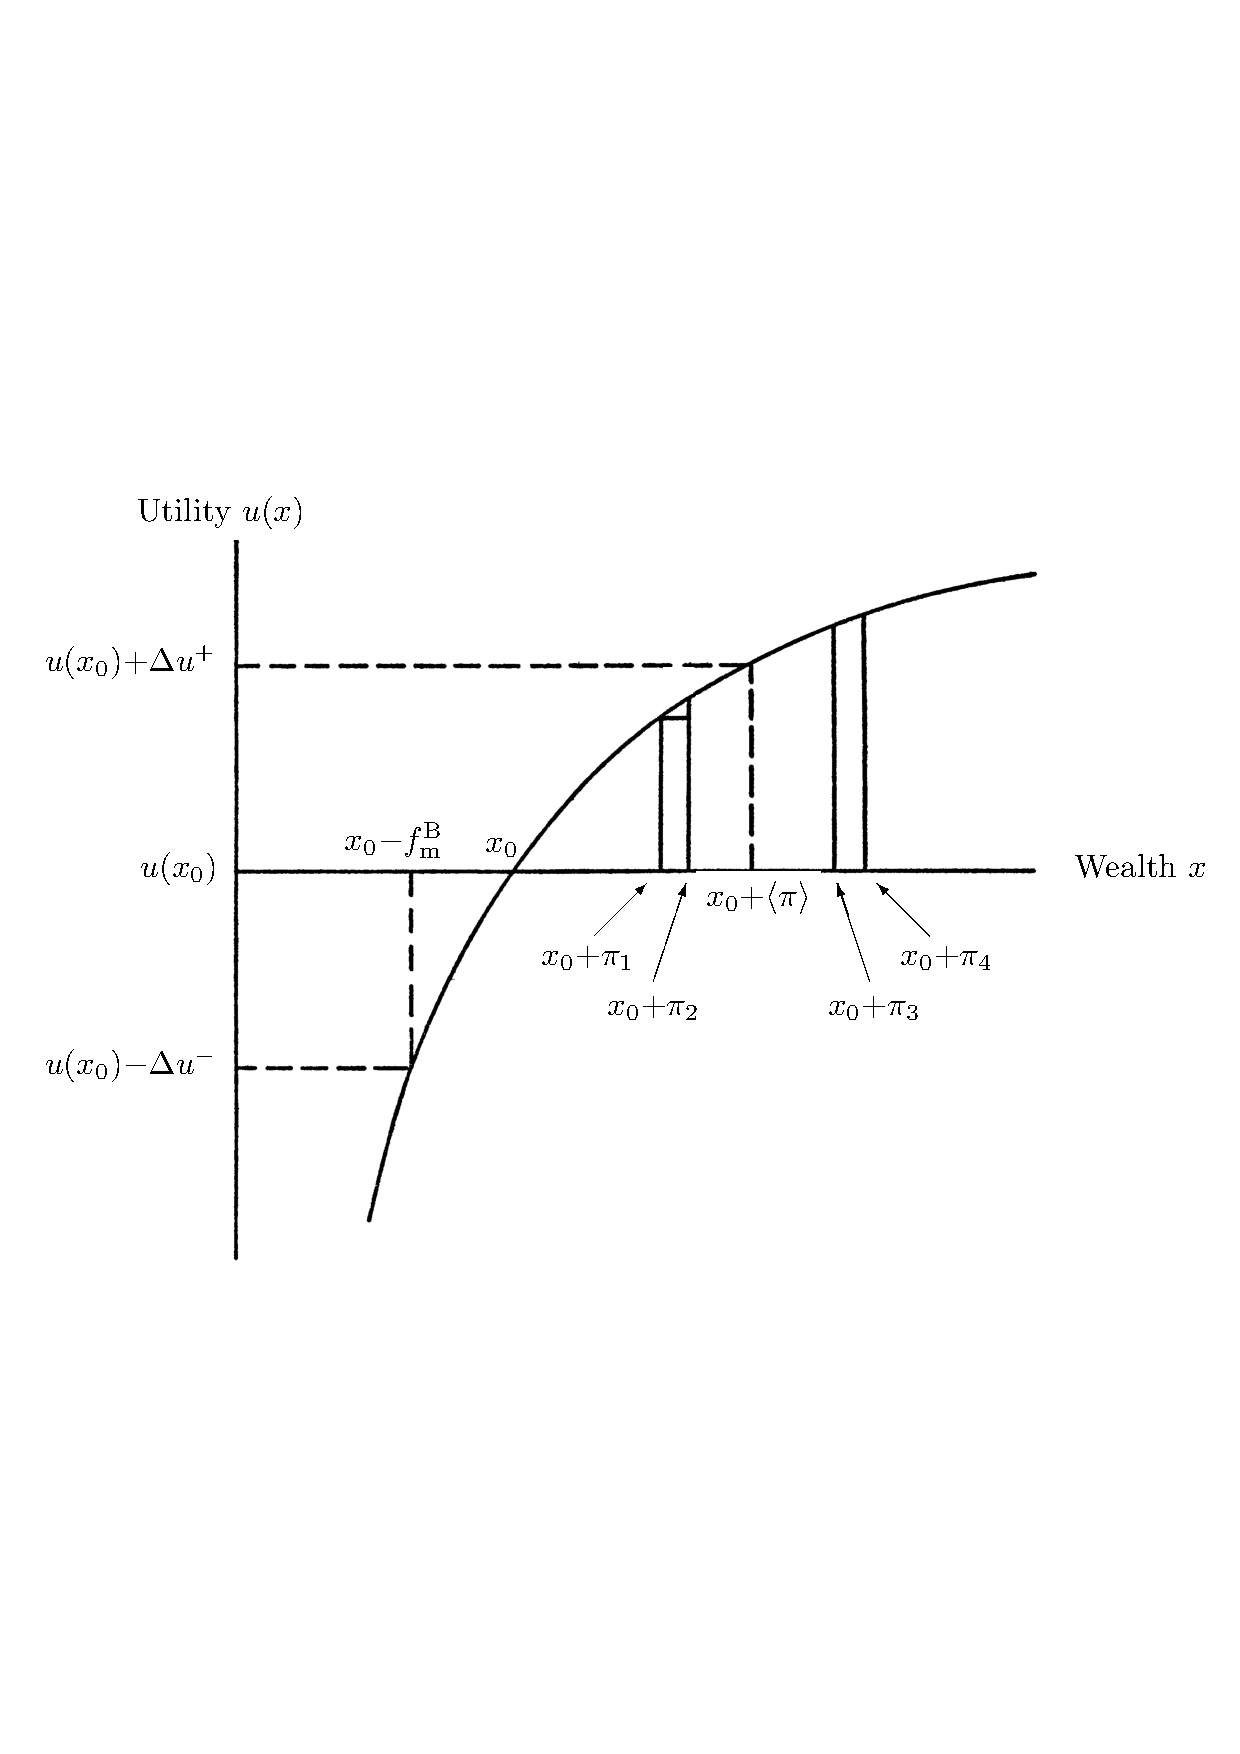
\includegraphics[width=.48\textwidth]{./new_notation.pdf}}
\end{picture}
& 
\begin{picture}(200,100)(5,20)
  \put(0,0){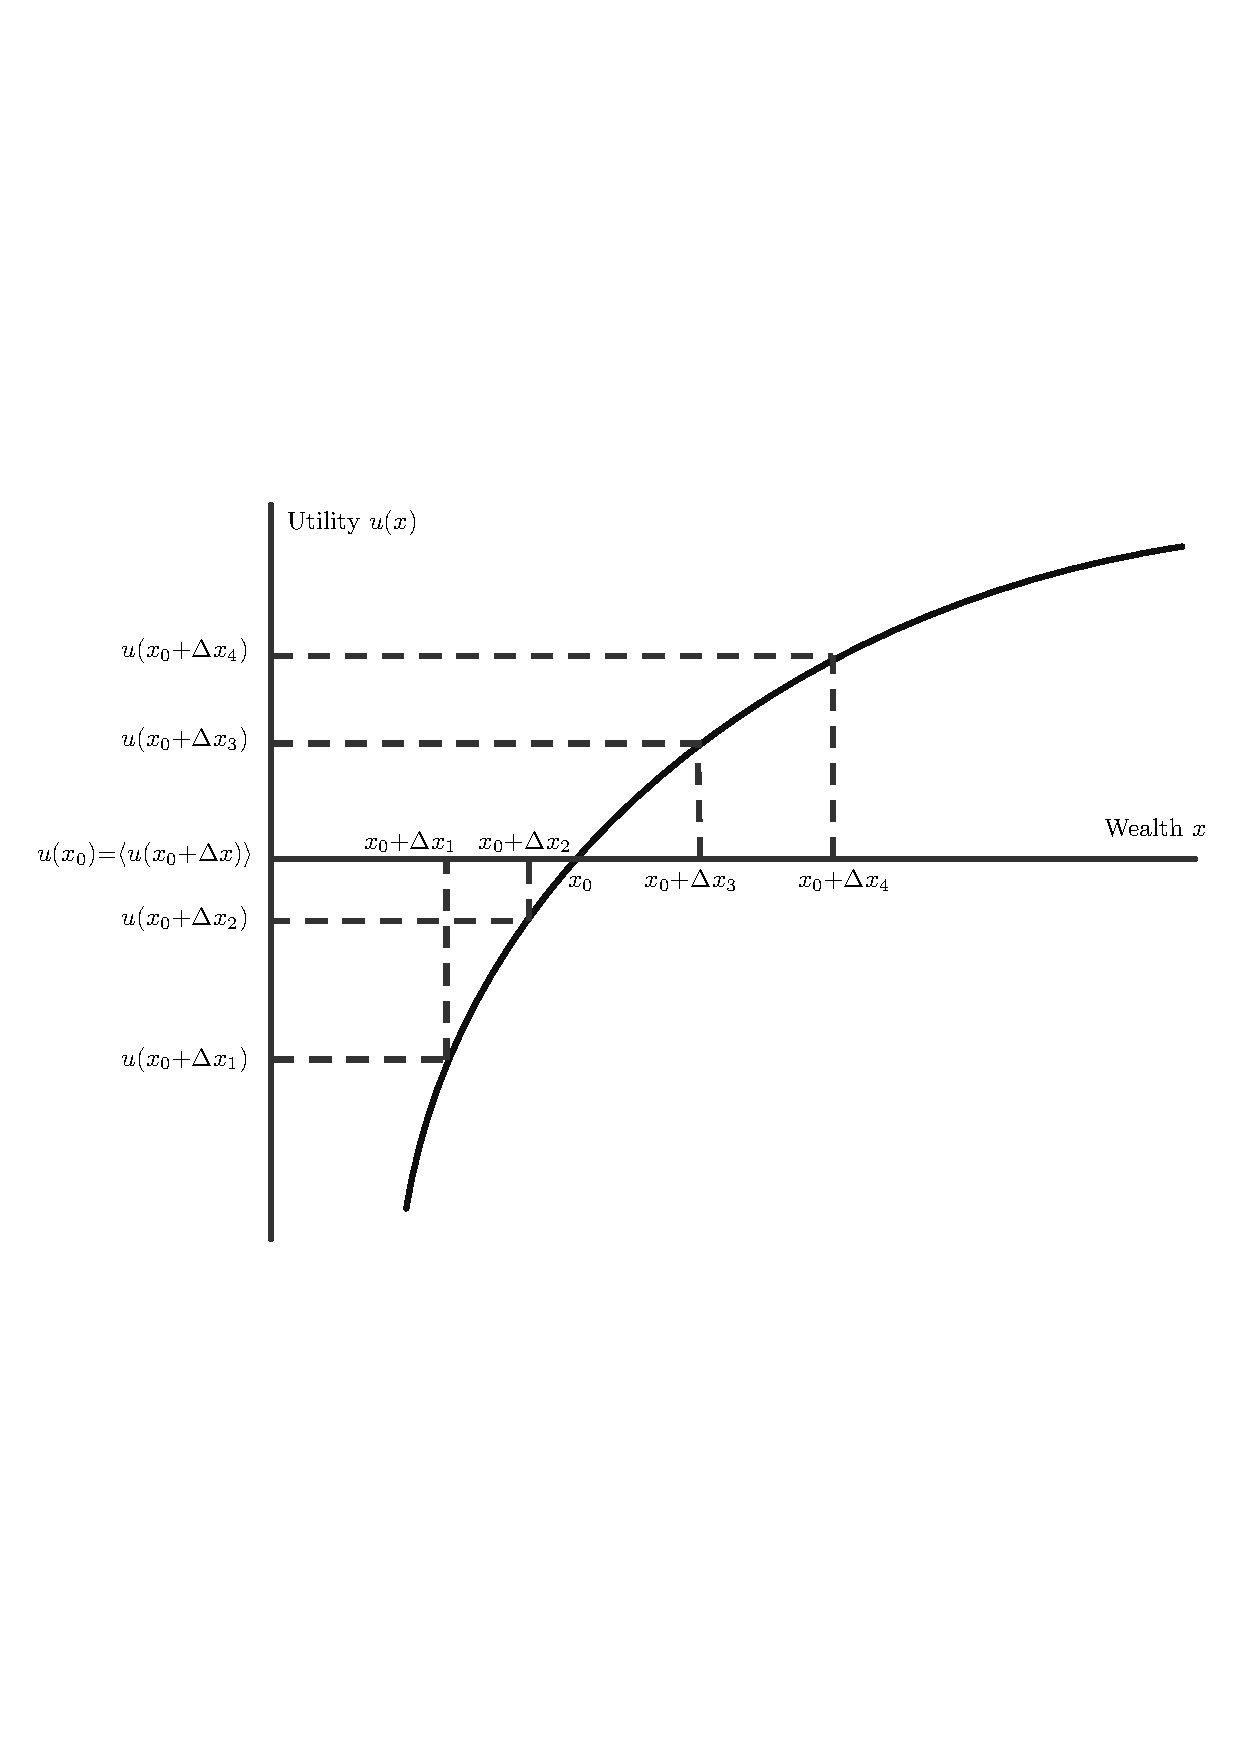
\includegraphics[width=.48\textwidth]{./EUT_exp.pdf}}
\end{picture} \\
    \tlabel{difference}
  \end{tabular}
\caption{Maximum fee to be paid for a lottery ticket, where prize $\pi_i$ is won with probability $p_i$, wealth $x$, initial wealth $x_0$, and utility function $u(x)$. {\bf The decision theory put forward by Bernoulli in 1738 is not expected utility theory (EUT).} Bernoulli did not compute the expected change in utility, whereas this is the object that determines the value of a lottery under EUT. Bernoulli's geometric construction does not correspond to EUT, and consequently the maximum fee computed by Bernoulli, $\tmb$, differs from the maximum fee according to EUT, $\tml$. EUT works with net changes in wealth, $\Dx_i=\pi_i-f$, whereas Bernoulli works with prizes, $\pi_i$, treating the fee, $f$, separately. The two theories constitute different mathematical models of human decision-making.}
\end{table}
\end{center}


Only a linear utility function guarantees the equality $\tmb=\tml$. In other words, Bernoulli's decision theory, which is often wrongly presented as equivalent to EUT, is really only equivalent to EUT under the assumption of linear utility. But that is equivalent to Huygens's decision theory that we encountered in \secref{Historical}, and that was deemed an unrealistic model of human behavior. 

Bernoulli's equation on his p.~26 is accompanied by a figure, reproduced in \fref{key}. The figure is not part of the original manuscript but was produced by Sommer and Menger. It is a clear illustration that Bernoulli's decision theory is not only inconsistent with EUT but indeed questionable in itself. Here is why: the maximum fee to be paid is represented in the figure by the length pB ($\tm$). This length is clearly less than the length BC ($\pi_1$) that represents the minimum prize to be received from playing the lottery\footnote{The types of lotteries considered by Bernoulli always result in receiving some prize, \ie it is not possible to receive nothing in return for the fee. For example, in the famous St. Petersburg lottery (the focus of Bernoulli's paper), at least \$1 is paid out (or one ducat in Bernoulli's currency).}. The minimum net change in wealth, \ie the worst possible result from playing the lottery, is thus $\pi_1-\tm>0$, which is positive. This lottery represents a guaranteed win of at least $\pi_1-\tm$ and possibly much more. There is no good reason to reject it, and a theory that predicts people would reject it will soon be falsified by observation. Ask the person next to you if he'd like to play the following gamble: toss a coin, and if heads shows the person gets \$20, if it's tails he gets \$10.


%\begin{figure}
%\centering
%\begin{picture}(300,200)(0,0)
%  \put(-55,0){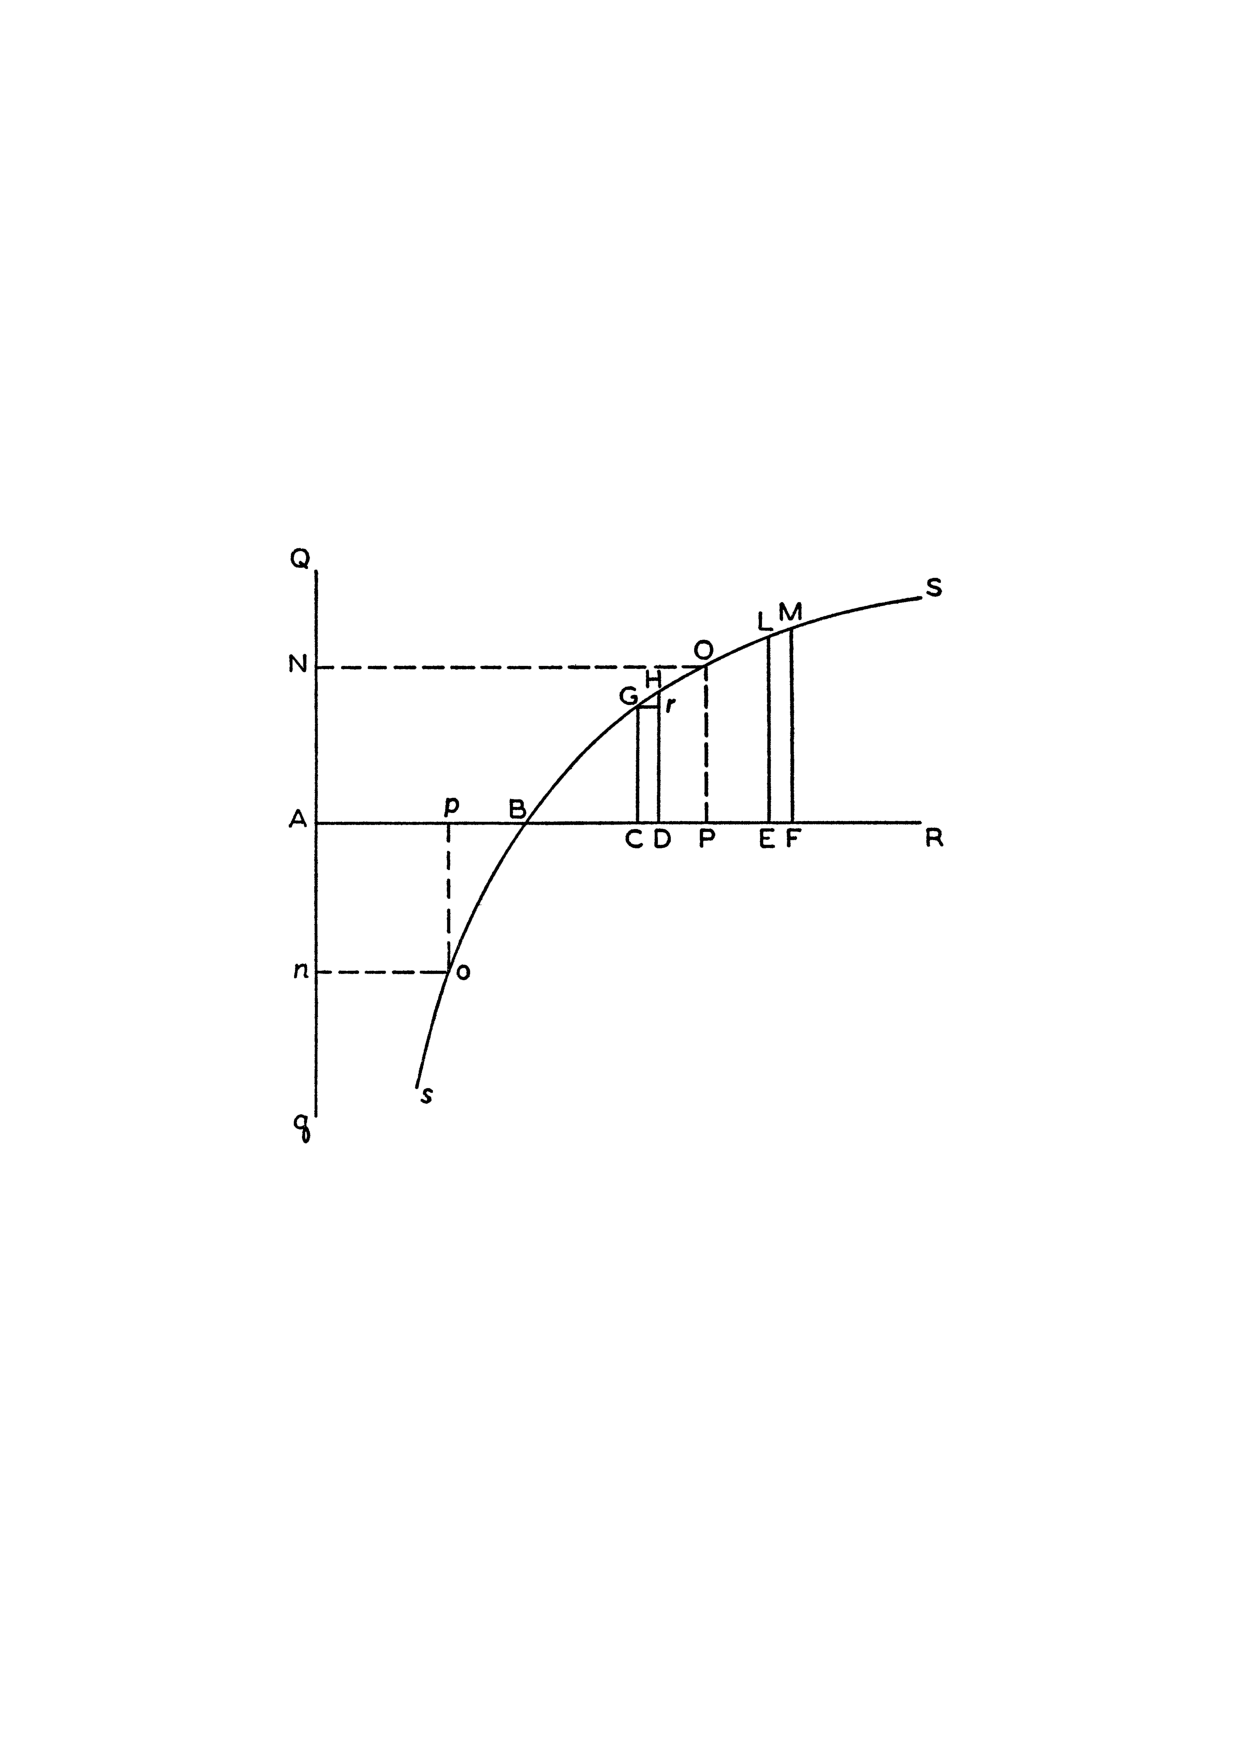
\includegraphics[width=.8\textwidth]{./Bernoulli1738.pdf}}
%\put(-55,245){\colorbox{white}{Utility $u(x)$}}
%\put(-54,137){\colorbox{white}{$u(x_0)$}}
%\put(-83,199.5){\colorbox{white}{$\mathbin{{u(x_0)}{+}{\Du^+}}$}}
%\put(-83,77){\colorbox{white}{$\mathbin{{u(x_0)}{-}{\Du^-}}$}}
%%delete q
%\put(-33,19){\colorbox{white}{~}}
%\put(-31,16){\colorbox{white}{~}}
%\put(-31,12){\colorbox{white}{~}}
%%delete s
%\put(20,30){\colorbox{white}{~}}
%\put(18,25){\colorbox{white}{~}}
%%delete o
%\put(34,80){\colorbox{white}{~}}
%\put(34,75){\colorbox{white}{~}}
%%delete C,D,P,E,F,R
%\put(90,134){\colorbox{white}{\hspace{5cm}}}
%\put(90,130){\colorbox{white}{\hspace{5cm}}}
%%delete G
%\put(98.5,192){\colorbox{white}{~}}
%\put(98.5,190){\colorbox{white}{~}}
%\put(98,189.5){\colorbox{white}{~}}
%\put(96.5,188.5){\colorbox{white}{~}}
%%delete H
%\put(108,197.7){\colorbox{white}{~}}
%\put(107.5,195.6){\colorbox{white}{~}}
%%delete r
%\put(118,189){\colorbox{white}{~}}
%\put(118,185){\colorbox{white}{~}}
%%delete O
%\put(128.5,207.5){\colorbox{white}{~}}
%\put(128.5,211){\colorbox{white}{~}}
%\put(127,206.7){\colorbox{white}{~}}
%%delete L
%\put(154,221){\colorbox{white}{~}}
%\put(154,218.5){\colorbox{white}{~}}
%%delete M
%\put(163,227){\colorbox{white}{~}}
%\put(163,222){\colorbox{white}{~}}
%\put(165,228){\colorbox{white}{~}}
%\put(164,223){\colorbox{white}{~}}
%%delete S
%\put(222.2,235){\colorbox{white}{~}}
%\put(222.2,230){\colorbox{white}{~}}
%\put(8,145){\colorbox{white}{$\mathbin{{x_0}{-}{\tmb}}$}}
%\put(53.3,143.2){\colorbox{white}{~}}
%\put(53.5,146.3){\colorbox{white}{~}}
%\put(54,144.5){$x_0$}
%\put(118,128){\colorbox{white}{$\mathbin{{x_0}{+}{\ave{\pi}}}$}}
%\put(68,110){\colorbox{white}{$\mathbin{{x_0}{+}{\pi_1}}$}}
%\put(87,119){\vector(1,1){16}}
%\put(88,95){\colorbox{white}{$\mathbin{{x_0}{+}{\pi_2}}$}}
%\put(105,105){\vector(1,3){10}}
%\put(177,110){\colorbox{white}{$\mathbin{{x_0}{+}{\pi_4}}$}}
%\put(189,119){\vector(-1,1){16}}
%\put(155,95){\colorbox{white}{$\mathbin{{x_0}{+}{\pi_3}}$}}
%\put(171,105){\vector(-1,3){10}}
%\put(230,137){\colorbox{white}{Wealth $x$}}
%\end{picture}
%\caption{\small A) Figure representing Bernoulli's 1738 computation of the maximum fee to be paid for a lottery. B) the same figure translated into modern notation. In Bernoulli's EUT, unlike in modern EUT, the maximum fee to be paid for a gamble is found as follows: find 1) the gain in utility, $\Du^+$ that would arise from receiving the expectation value of the prize (disregarding the fee). Find 2) the fee such that the loss in utility that would arise from paying it without receiving any prize, $\Du^-$ is the same as $\Du^+$. This contradicts modern utility theory where the maximum fee is the fee that renders the expectation value of the change in utility due to net changes in wealth zero, $\ave{\Du}=0$.}
%\flabel{key}
%\end{figure}
%
%\begin{figure}
%\centering
%\begin{picture}(300,500)(0,0)
%  \put(-10,200){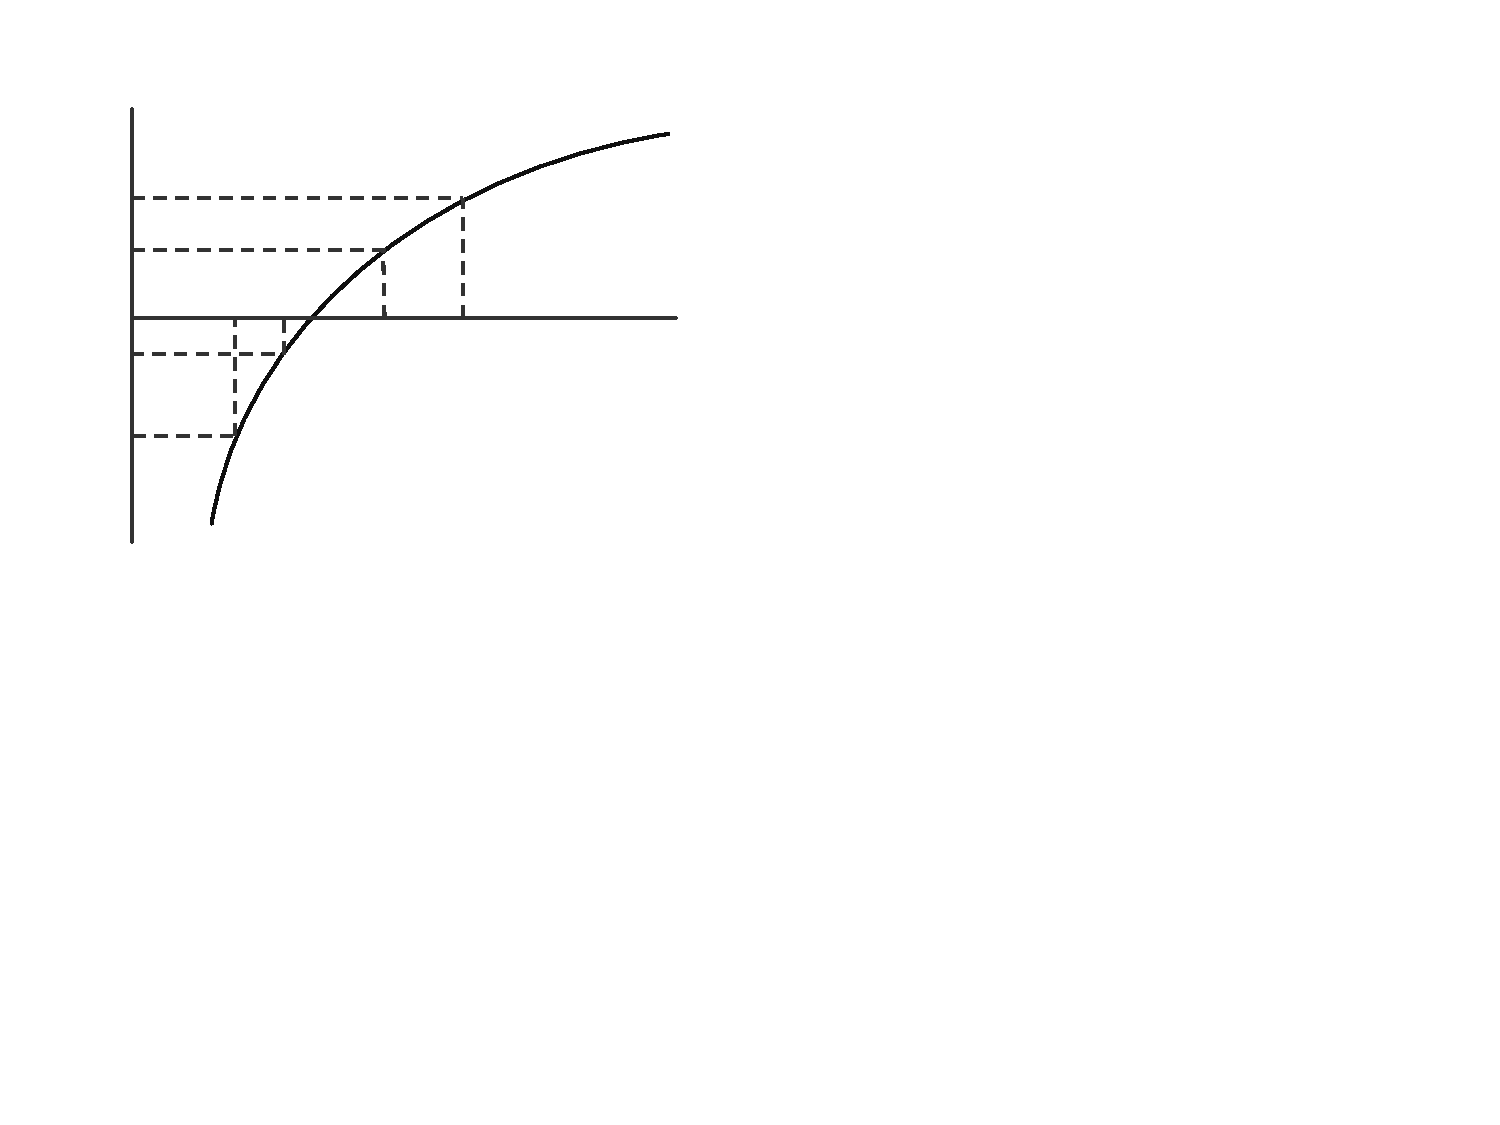
\includegraphics[width=\textwidth]{./EUT_curve.pdf}}
% \put(40,360){$\mathbin{{x_0}{+}{\Dx_1}}$}
% \put(85,360){$\mathbin{{x_0}{+}{\Dx_2}}$}
% \put(120,345){$x_0$}
% \put(150,345){$\mathbin{{x_0}{+}{\Dx_3}}$}
% \put(210,345){$\mathbin{{x_0}{+}{\Dx_4}}$}
% \put(-55,435){$\mathbin{{u(x_0}{+}{\Dx_4)}}$}
% \put(-55,400){$\mathbin{{u(x_0}{+}{\Dx_3)}}$}
% \put(-88,355){$\mathbin{{u(x_0)}{=}{\ave{u(\mathbin{{x_0}{+}{\Dx)}}}}}$}
% \put(-55,330){$\mathbin{{u(x_0}{+}{\Dx_2)}}$}
% \put(-55,275){$\mathbin{{u(x_0}{+}{\Dx_1)}}$}
% \put(10,485){Utility $u(x)$}
% \put(330,365){Wealth $x$}
%\end{picture}
%\caption{Modern EUT.}
%\flabel{key}
%\end{figure}



\begin{figure}
\centering
\begin{picture}(300,400)(0,0)
 \put(-20,380){A)}
  \put(5,200){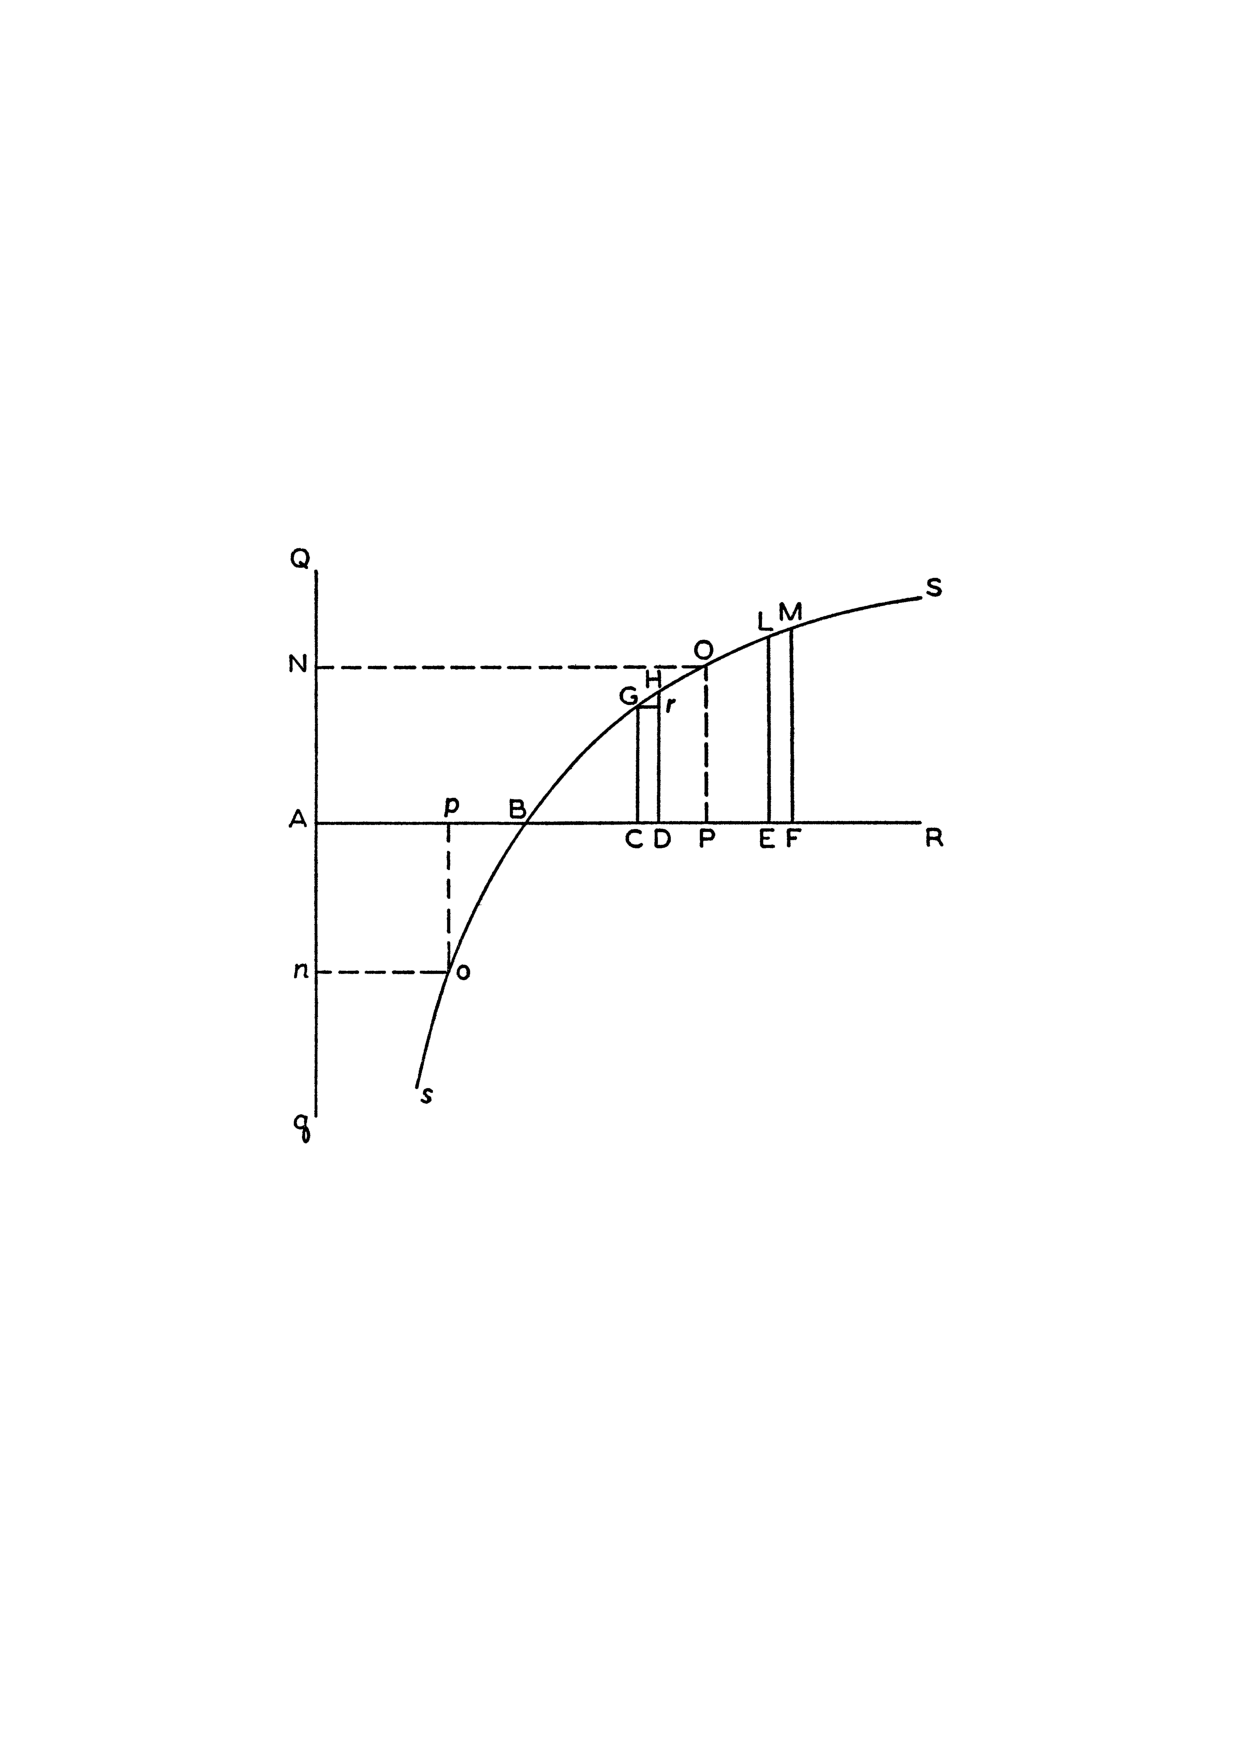
\includegraphics[width=.6\textwidth]{./Bernoulli1738.pdf}}
 \put(-20,173){B)}
  \put(-24,-100){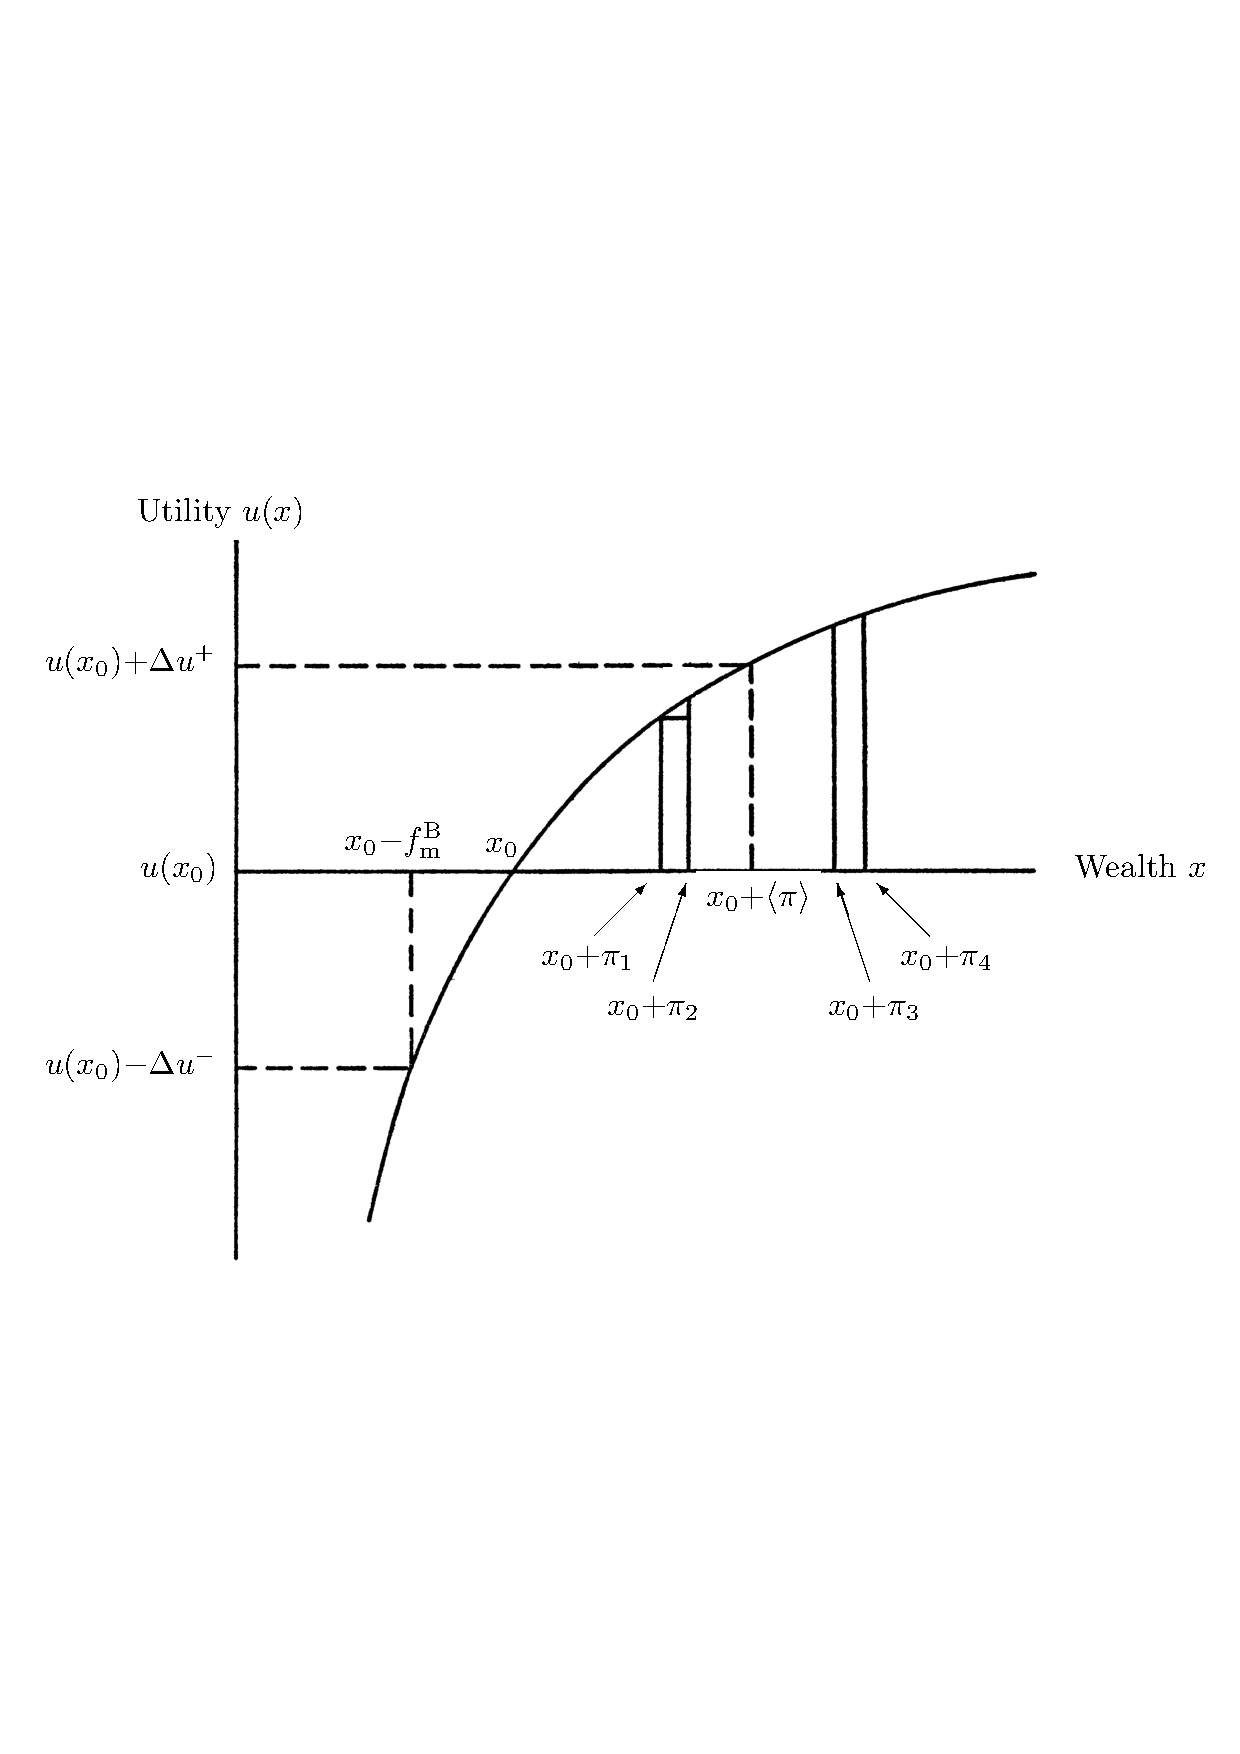
\includegraphics[width=.73\textwidth]{./new_notation.pdf}}
\end{picture}
\caption{\small  A) Bernoulli's 1738 computation of the maximum fee to be paid for a lottery. B) the same figure translated into modern notation. In Bernoulli's decision theory, unlike in modern EUT, the maximum fee to be paid for a gamble is found as follows: find 1) the gain in utility, $\Du^+$ that would arise from receiving the expectation value of the prize (disregarding the fee). Find 2) the fee such that the loss in utility that would arise from paying it without receiving any prize, $\Du^-$ is the same as $\Du^+$. This contradicts modern utility theory where the maximum fee is the fee that renders the expectation value of the change in utility due to net changes in wealth zero, $\ave{\Du}=0$.}
\flabel{key}
\end{figure}


\section{Discussion}
\seclabel{Discussion}
It is impossible to reconcile BDT with EUT. 
We are, however, free to speculate about the reasons for Bernoulli's inelegant theory. It is possible that Bernoulli developed a different decision theory on purpose. He proposed a different model of human psychology, and perhaps he meant to do just that. Over the centuries, as we learned more about stochastic systems, we diverged from his original vision. 

We may also suggest that Bernoulli made a sloppy error; in effect a typo. This is not a likely scenario, due to Bernoulli's consistent use of \eref{ub} throughout his paper. A sloppy error would most likely occur in just one place.

A third interpretation is that the difference between BDT and EUT is a more serious confusion on Bernoulli's part about the early mathematical concept that is the expectation value. In this reading,  Bernoulli actually wanted to compute $\ave{\Du}$ but didn't notice that his computation did not achieve this. This interpretation is supported by the following passage \cite[p.~24]{Bernoulli1738}: ``Meanwhile, let us use this as a fundamental rule: If the utility of each possible profit expectation is multiplied by the number of ways in which it can occur, and we then divide the sum of these products by the total number of possible cases, a mean utility will be obtained, and the profit which corresponds to this utility will equal the value of the risk in question.'' This strongly suggests that Bernoulli wanted to compute $\ave{\Du}$, and indeed this is how Laplace interpreted it when he claimed that Bernoulli had proposed to compute $\ave{\Du}$. Laplace omitted the information that his claim implies that Bernoulli made an error. This scenario is not unlikely, given the state of probability theory at the time of Bernoulli's writing. But the absence of an equation at \cite[p.~24]{Bernoulli1738} leaves the statement open to interpretation. The following interpretations would make this statement equivalent to modern EUT and contradict Bernoulli's BDT: 
\bi
\item
Bernoulli meant ``net profit'' when he wrote ``profit,'' including losses as negative profits. 
\item
He meant to restrict the statement to risks that require no fee to participate.
\ei

On the other hand, another plausible interpretation would keep Bernoulli's statement here consistent with the rest of his paper but inconsistent with modern EUT:
\bi
\item
By ``profit'' Bernoulli means ``prize,'' disregarding the fee.
\ei

Laplace presents modern EUT that computes $\ave{\Du}$ as a criterion for gamble participation and ascribes it to Bernoulli, omitting the fact that Bernoulli actually put forward a different theory and did not compute this object. If the inconsistency between Bernoulli and the far more natural modern form of EUT seems astonishing, we should remind ourselves of how early in the development of probability theory, mathematics, and of course economics Bernoulli's study sits. Probability theory was in its infancy (Kolmogorov's axioms of 1933 \cite{Kolmogorov1933} are often considered the foundation of modern probability theory). The key concept Bernoulli stumbles over was in the process of being developed in the 18th century. This concept is the following:  a function of a random value, such as $u(x)$, defines a new random variable (see \secref{Mathematical}) whose expectation value is not trivially related to the expectation value of $X$, namely $\ave{u(x)}\neq u(\ave{x})$, and $\ave{\Du(x)}\neq u(\ave\Dx)$ \etc As an illustration of the historical mathematical context, let's remember that this complication is behind Bertrand's circle problem \cite{Bertrand1889}, put forward as late as 1889 in response to Laplace's flawed ``principle of insufficient reason'' of 1812, which it exposes as invalid, see the discussion in \cite[p.~20]{vanKampen2007}.

It is my impression that the inconsistency between Bernoulli's decision theory and modern EUT has caused a great deal of confusion. For instance, Karl Menger's famous result that utility functions must be bounded \cite{Menger1934} makes use of Bernoulli's original work and falls apart when one tries to derive it from modern EUT \cite{Peters2011c,PetersGell-Mann2016}. Campbell notes that this result is now ``routinely ignored'' \cite[p.~5]{Campbell2017}, yet it persists in the literature without a retraction of, or comment on, the original paper. Similarly, discussions of prospect theory and cumulative prospect theory often confusingly claim that EUT does not contain a reference value. The reference value in EUT is present wealth, $x_0$. The confusion may be related to the problem under investigation: if we insist that Bernoulli's and modern EUT are equivalent, we are forced to assume linear utility, and in that special case the reference value, $x_0$, cancels out from the computation of the decision criterion $\ave{\Du}$ in \eref{EUT}.

A clear understanding of Bernoulli's work and its deviations from modern EUT prevents this sort of confusion. It leads to an interpretation of EUT in terms of ergodicity transformations that has proved very useful recently, shedding new light on long-standing problems in economic theory, including the St. Petersburg paradox, the cooperation conundrum, and the equity premium puzzle.

\bibliographystyle{plain}
\bibliography{bibliography}
\end{document}

